This subsection describes the experiments that uncovers the best combination of hidden layers, neurons and epochs as well as the different strategies. Based on the above analysis of wind production influences the network will be tested with combinations of the following input parameters:

\begin{itemize}
\item Wind speed;
\item Air density;
\item Consumption;
\item Time of day;
\item Temperature;
\item Wind direction;
\item Last known production;
\item Date;
\end{itemize}

Furthermore, experiments are needed to investigate the influence of data manipulation and statistical inputs as presented in Section~\ref{sec:usingStatisticalInput}. 

\todo{DRAWING OF NETWORK}

\subsection{Experiment Series One - Selection of input parameters}
The first experiment series is an attempt to find the best constitution of network input parameters based on the analysis in Section~\ref{sec:windPowerAnalysis}. All test results can be seen in Appendix~\ref{sec:windResultsAppendix} and have been carried out naively with only normalization - relevant results will be shown here. Since the co-relation between wind production and wind speed is very significant it will always be included as a core input parameter in all test combinations.

\footnotesize
\begin{center}
\begin{longtable}{|c|c|c|c|c|c|c|c|c|c|}
\hline
\textbf{WS} & \textbf{AD} & \textbf{C} & \textbf{T} & \textbf{WD} & \textbf{L-P} & \textbf{Mo}& \textbf{ToD} & \textbf{MAE} & \textbf{Rank} \\
\hline
\endfirsthead
\multicolumn{10}{c}%
{\tablename\ \thetable\ -- \textit{Continued from previous page}} \\
\hline
\textbf{WS} & \textbf{AD} & \textbf{C} & \textbf{T} & \textbf{WD} & \textbf{L-P} & \textbf{Mo}& \textbf{ToD} & \textbf{MAE} & \textbf{Rank} \\
\hline
\endhead
\hline \multicolumn{10}{r}{\textit{Continued on next page}} \\
\endfoot
\hline
\endlastfoot
\arrayrulecolor{light-gray}
 \x &  &  &  \x &  &  \x &  &  \x & 127.86 & \#1 \\ \hline
 \x &  \x &  &  &  \x &  \x &  &  \x & 131.59 & \#2 \\ \hline
 \x &  \x &  &  &  &  \x &  &  \x & 131.89 & \#3 \\ \hline
 \x &  \x &  \x &  \x &  \x &  \x &  &  \x & 133.18 & \#4 \\ \hline
 \x &  \x &  \x &  \x &  \x &  \x &  &  & 133.77 & \#5 \\ \hline
 \x &  \x &  \x &  &  &  \x &  &  \x & 134.14 & \#6 \\ \hline
 \x &  \x &  \x &  &  \x &  \x &  &  \x & 135.4 & \#7 \\ \hline
 \x &  \x &  \x &  &  &  \x &  &  & 136.33 & \#8 \\ \hline
 \x &  \x &  &  &  &  \x &  \x &  \x & 136.65 & \#9 \\ \hline
 \x &  &  &  &  &  \x &  &  & 137.33 & \#10 \\ \hline
 . & . & . & . &  .  & . &  . & . & . & . \\ 
 . & . & . & . &  .  & . &  . & . & . & . \\ 
 . & . & . & . &  .  & . &  . & . & . & .\\ \hline
 \x &  \x &  &  \x &  &  \x &  \x &  & 170.93 & \#119 \\ \hline
 \x &  &  \x &  \x &  \x &  \x &  \x &  \x & 171.61 & \#120 \\ \hline
 \x &  &  \x &  \x &  &  \x &  \x &  & 172.72 & \#121 \\ \hline
 \x &  &  &  &  \x &  \x &  \x &  & 173.12 & \#122 \\ \hline
 \x &  &  \x &  \x &  &  \x &  \x &  \x & 173.65 & \#123 \\ \hline
 \x &  \x &  \x &  \x &  \x &  \x &  \x &  \x & 174.26 & \#124 \\ \hline
 \x &  \x &  &  \x &  &  \x &  \x &  \x & 174.55 & \#125 \\ \hline
 \x &  &  &  \x &  &  \x &  \x &  \x & 174.85 & \#126 \\ \hline
 \x &  \x &  \x &  &  \x &  \x &  \x &  & 180.89 & \#127 \\ \hline
 \x &  \x &  &  &  \x &  \x &  \x &  \x & 199.22 & \#128 \\ \hline
\caption{Wind Production Input Parameter Test Top and bottom 10. It is based on 3 month of historical data and 200 epochs. It is an average of the prediction over 8000 hours}
\end{longtable}
\label{table:windProdInputParamsTop10}
\end{center}
\normalsize

All results from the first experiment can be seen in Appendix~\ref{sec:simpleInputTest}. The results vary from the best MAE at 127,86 to the worst being 199,22. Top and bottom 10 is shown in Table~\ref{table:windProdInputParamsTop10} indicated by rank. The experiment clearly shows the importance of time of day and last production. This correspond well with the analysis in Section~\ref{sec:windPowerAnalysis} where the relationship between wind production and the parameters are established to be significant. Especially the analysis concerning the importance of wind production development is  seen in the experiments. The production does not differ much from one hour to the next which is reflected in the last known production input parameter --- more sophisticated attempts with statistic will be in experiments to come. It is also seen in the bottom 10 that when put together with conflicting parameters the last production does not contribute enough.  What comes as a surprise is the under representation of consumption in top 10 because the analysis showed a good co-relation. A possible explanation can be bad co-relation between consumption and some of the other input parameters that makes more noise and influence the prediction badly. The analysis section also discussed the substitution of temperature with consumption --- this can be what is seen in \#1. Temperature is also the significant factor in calculating air density because pressure is close to constant as described in Section~\ref{sec:airDensity} --- this can explain why \#1 is the only one in top 9 without air density. Furthermore it can explain why consumption can be substituted with air density since it is based on the temperature.

Wind Direction is represented four times in top 10. What is noticeable is the same combinations without wind direction is also represented which indicates the indifference of wind direction, e.g. see \#2-\#3 and \#6-\#7. This is further backed up by the analysis which only showed a low co-relation. 

What is obvious from the experiment is the impact of month as input parameter and how it in general does not help the prediction. What comes to mind is the historical data used for testing. Month represents the seasonal perspective and is suppose to find the relationship between months and the production in general. Since the historical data used for prediction is only 3 months, it does not capture how months in general influenced the production in the past year. A possible solution to obtain the seasonality aspect is presented in\cite{pjmForecast} where the Neural Network is trained with 45 days from before the day to be predicted, and 45 days before and after in the previous year. By using this approach the month parameter will reflect the influence of the months around you from the last year. This needs validation in an experiment for itself. The experiment results can be seen in Table~\ref{table:seasonalWindProdInputParamsTop10}. What is clear is the immediate decrease in MAE. This can be explained by the increase data in the training set that makes it harder for the ANN to generalize. According to\cite{1} too large training sets should be avoided because it has a tendency to be overtrained. The possible benefits from including the seasonal aspect when predicting wind production can not make up for the loss in accuracy by the increase in the size of training data. To further validate the decrease in accuracy when using season and a larger dataset, another test on an entire year has been conducted for \#6 in Table~\ref{table:seasonalWindProdInputParamsTop10}. The result can be seen in Table~\ref{table:seasonWindProdInputParamsTop2WholeYear}. The MAE is around the same but instead it takes longer time to run it on an entire year. This makes the small dataset a better choice. The usage of only 3 months in the dataset can be argued to contain the seasonal aspect for the hours to predict. The three months in the set will reflect the current season that you are in and therefore adding more data will only create more noise. The month parameter will not say anything about the past year but instead the months it has already seen --- it will reflect how the past 3 month impacted the price, but also include the transitions between the months / seasons. It needs to be made clear that it is only worsened with 10 in average and it is only one input parameter of the entire network. The above discussion clearly illustrates that the small data itself contains the seasonality because the network trains and generalizes only upon the current season. For this reason the month parameter will be omitted in the prediction of wind production --- this is also clear when looking at Table~\ref{table:windProdInputParamsTop10} where only \#9 is with month and all of bottom 10 is with. \todo{argument and compare curves from 2012 and 2011}. 

In experiments concerning prediction of wind production the month input parameter will be left out.  

\footnotesize
\begin{center}
\begin{longtable}{|c|c|c|c|c|c|c|c|c|c|}
\hline
\textbf{WS} & \textbf{AD} & \textbf{C} & \textbf{T} & \textbf{WD} & \textbf{L-P} & \textbf{Mo}& \textbf{ToD} & \textbf{MAE} & \textbf{Rank} \\
\hline
\endfirsthead
\multicolumn{9}{c}%
{\tablename\ \thetable\ -- \textit{Continued from previous page}} \\
\hline
\textbf{WS} & \textbf{AD} & \textbf{C} & \textbf{T} & \textbf{WD} & \textbf{L-P} & \textbf{Mo}& \textbf{ToD} & \textbf{MAE} & \textbf{Rank} \\
\hline
\endhead
\hline \multicolumn{9}{r}{\textit{Continued on next page}} \\
\endfoot
\hline
\endlastfoot
\arrayrulecolor{light-gray}
 \x &  \x &  \x &  &  \x &  \x &  &  \x & 142.88 & \#1 \\ \hline
 \x &  &  &  \x &  \x &  \x &  &  & 142.89 & \#2 \\ \hline
 \x &  \x &  &  &  \x &  \x &  &  \x & 143.37 & \#3 \\ \hline
 \x &  \x &  \x &  \x &  \x &  \x &  &  \x & 143.97 & \#4 \\ \hline
 \x &  &  &  &  &  \x &  &  \x & 143.98 & \#5 \\ \hline
 \x &  \x &  \x &  \x &  &  \x &  \x &  & 144.11 & \#6 \\ \hline
 \x &  \x &  &  &  &  \x &  &  & 144.12 & \#7 \\ \hline
 \x &  &  &  &  &  &  &  \x & 144.28 & \#8 \\ \hline
 \x &  &  \x &  &  \x &  \x &  &  & 144.42 & \#9 \\ \hline
 \x &  \x &  &  \x &  \x &  \x &  &  \x & 144.48 & \#10 \\ \hline
\caption{Top 10 seasonal wind production test. It is based on 3 month of historical data and one month after from the previous year. It is run with 200 epochs and predicts 8000 hours in 2012}
\end{longtable}
\label{table:seasonalWindProdInputParamsTop10}
\end{center}
\normalsize



\todo{trend discussion in relation to why seasonal impl is better on small dataset}.

\footnotesize
\begin{center}
\begin{longtable}{|c|c|c|c|c|c|c|c|c|c|}
\hline
\textbf{WS} & \textbf{AD} & \textbf{C} & \textbf{T} & \textbf{WD} & \textbf{L-P} & \textbf{Mo}& \textbf{ToD} & \textbf{MAE} & \textbf{Rank} \\
\hline
\endfirsthead
\multicolumn{9}{c}%
{\tablename\ \thetable\ -- \textit{Continued from previous page}} \\
\hline
\textbf{WS} & \textbf{AD} & \textbf{C} & \textbf{T} & \textbf{WD} & \textbf{L-P} & \textbf{Mo}& \textbf{ToD} & \textbf{MAE} & \textbf{Rank} \\
\hline
\endhead
\hline \multicolumn{9}{r}{\textit{Continued on next page}} \\
\endfoot
\hline
\endlastfoot
\arrayrulecolor{light-gray}
 \x &  \x &  \x &  \x &  &  \x &  \x &  & 147.98 & \#6 \\ \hline
\caption{Seasonal wind production test based on an entire year. It is run with 200 epochs and predicts 8000 hours in 2012}
\end{longtable}
\label{table:seasonWindProdInputParamsTop2WholeYear}
\end{center}
\normalsize
\todo{see appendix}


The three best ranked combination of parameters will be the basis for all coming experiments --- we assume that 8000 hours of prediction can be characterized as general. The prediction for the first 175 hours of the best from Table~\ref{table:windProdInputParamsTop10} can be seen in Figure~\ref{fig:bestInputParameterPrediction}. It can be observed that the prediction follows the trend of the actual wind production. The obvious challenge is that the prediction takes time to identify shifting trend --- either it identifies it before happens or after it happened. From hour 25-50 it is way behind the actual slope. It can also be seen around hour 100-110 that it significantly overshoots and in 120-160 undershoots its target before actually identifying the shift. The statistical approach described in Section~\ref{sec:usingStatisticalInput} can possible help in these cases by taking current trend into consideration. Experiments will take up this approach for comparison.  

\begin{figure}[H]
\centering
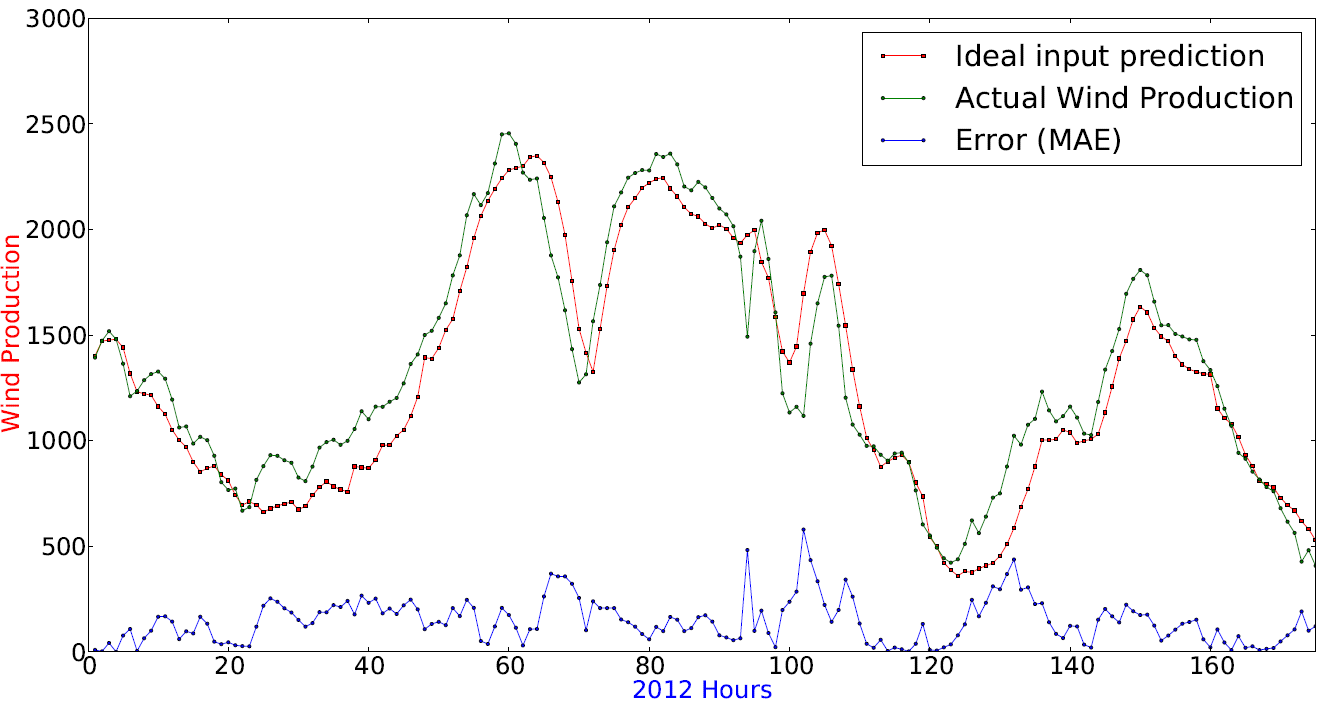
\includegraphics[width=0.99\linewidth]{billeder/bestInputParameterPrediction.png}
\caption{Wind production prediction for 175 hours in 2012}
\label{fig:bestInputParameterPrediction}
\end{figure}   

The experiments to come will be based on input combinations from the top 3 from Table~\ref{table:windProdInputParamsTop10}. The inputs are:
\begin{itemize}
\item Wind speed;
\item Air density;
\item Wind Direction;
\item Temperature;
\item Last known production;
\item Time of day;
\end{itemize}

\subsection{Experiment Two - Data Manipulation}
Trimming is only an issue if irregularities exist\todo{use curves to illustrate that it is not necessary here and make graph that shows that the top is cut off and it is not irregular in any way}. The purpose of the experiments in series two is to turn inputs into a matrix whenever possible. As described in Section~\ref{sec:Matrix} one input parameter is split into one input parameter for all of its possible values --- it makes sense because each input parameter then has a weight that is adjusting itself according to the error as illustrated in Section~\ref{sec:annSection}. This is of course only an option if all values are known in advance and of a manageable size. When considering wind production forecasting this is valid for hours of the day, month and wind speed. Wind speeds are represented  by 41 different speeds in our data set. Instead of having only one input to represent each of the values, we can have 41 inputs for every single one of them. The purpose is to have a weight that tells exactly how much the specific input parameter in general influence the wind production to predict. Whenever a specific value is inserted it will be indicated with 1 and the rest of the matrix with 0. The network will then be adjusting a weight for the different entrances in the matrix whenever they are seen. What can become a problem is if some values does not exist or are under-represented which will cause that specific value to be under-expressed and not able to cover unseen data because the weight has only been adjusted a few times or not at all. In theory the matrix manipulation makes the most sense when all values to some degree are equally distributed so that every input in the matrix can express all values equally. Consider the case where wind speed 5 is not represented in the training dataset but is in the prediction data set. The network then won't have any clue how to relate to 5 when using the matrix implementation. In this case it makes sense to use one input parameter as representation because one weight have been adjusted to all the other values and illustrates how they in general influence the wind production. With that information contained in the weight it can also express 5 when the two are multiplied. Hours of the day and months are of course equally distributed. This assumption is validated in Table~\ref{windProdInputParamsTop10WithMatrix} where matrix on the wind speeds are obviously a bad choice. 

\begin{center}
\begin{longtable}{|c|c|c|c|c|c|c|c|c|}
\hline
\textbf{WS} & \textbf{AD} & \textbf{C} & \textbf{T} & \textbf{WD} & \textbf{L-P} & \textbf{ToD} & \textbf{MAE} & \textbf{Rank} \\
\hline
\endfirsthead
\multicolumn{9}{c}%
{\tablename\ \thetable\ -- \textit{Continued from previous page}} \\
\hline
\textbf{WS} & \textbf{AD} & \textbf{C} & \textbf{T} & \textbf{WD} & \textbf{L-P} & \textbf{ToD} & \textbf{MAE} & \textbf{Rank} \\
\hline
\endhead
\hline \multicolumn{9}{r}{\textit{Continued on next page}} \\
\endfoot
\hline
\endlastfoot
\arrayrulecolor{light-gray}
 \x &  &  &  \x &  &  \x &  \x (m) &126.25 & \#1 \\ \hline
 \x &  \x &  &  &  &  \x &  \x (m) &127.95 & \#2 \\ \hline
 \x &  \x &  &  &  \x &  \x & \x (m) &130.07 & \#3 \\ \hline
 \x (m) & &  &  \x &  &  \x &  \x (m) &135.71 & \#4 \\ \hline
 \x (m) & \x &  &  &  \x &  \x &  \x & 144.44 & \#5 \\ \hline
  \x (m) & \x &  &  &  &  \x &  \x & 147.63 & \#6 \\ \hline
 \x (m) & \x &  &  &  \x &  \x &  \x (m) &149.18 & \#7 \\ \hline
 \x (m) & &  &  \x &  &  \x &  \x & 149.19 & \#8 \\ \hline
 \x (m) & \x &  &  &  &  \x &  \x (m) &155.46 & \#9 \\ \hline
\caption{Matrix test}
\end{longtable}
\label{table:windProdInputParamsTop10WithMatrix}
\end{center}

\todo{discuss how matrix both influence indirectly and directly influence the prediction. Both pros and cons. The point is that a new month will not be influenced by the month before in terms of the weight. It will have its own. You remove responsibility from the other weights, they do not have to incorporate fx. how the month influence, they can focus only on wind speed and how it relates to the output}

\subsection{Experiment Three - Calculated Inputs}
This subsection is experimenting with the concepts described in Section~\ref{sec:usingStatisticalInput}. The point is to add inputs that in some way analyse productions from past hours to help the existing generalization approach its target more accurately. We therefore see it as independent from the input analysis since it will help the best of the input combinations to perform better. All of the approaches takes outset in previous hours so the first step is to find the best number of hours to calculate upon. The different approaches are historical volatility, skewness, simple curve analysis and inclusion of previous productions as input. 

\subsubsection{Historical Volatility}
Historical Volatility is presented in Section~\ref{sec:usingStatisticalInput}. It will calculate the volatility of the productions from hour to hour. This means that the last hour in the training set will hold information of the volatility of the entire dataset. We will use the EWMA to calculate volatility \todo{ref it back} and here it is necessary to experiment with the correct decay rate. The EWMA will always include the last hours EWMA --- this is why it is called moving average. The test will be performed in the best MAE from last experiment. When the best rate has been established for hour dataset it will be tested on top 10 from Table~\ref{table:windProdInputParamsTop10} with and without matrix.

\begin{center}
\begin{longtable}{|c|c|}
\hline
\textbf{Devay} & \textbf{MAE} \\
\hline
\endfirsthead
\multicolumn{2}{c}%
{\tablename\ \thetable\ -- \textit{Continued from previous page}} \\
\hline
\textbf{Decay} & \textbf{MAE}\\
\hline
\endhead
\hline \multicolumn{2}{r}{\textit{Continued on next page}} \\
\endfoot
\hline
\endlastfoot
\arrayrulecolor{light-gray}
0,10 & 122,75 \\ \hline
0,30 & 125,49 \\ \hline
0,60 & 127,49 \\ \hline
0,70 & 127,97 \\ \hline
0,50 & 130,47 \\ \hline
0,20 & 134,06 \\ \hline
0,80 & 135,17 \\ \hline
0,40 & 137,21 \\ \hline
0,90 & 139,16 \\ \hline
\caption{Different decay rates for historical volatility}
\end{longtable}
\label{table:historicalVoltalityHours}
\end{center}

\subsubsection{Skewness}
Skewness is a calculation of how much a distribution leans to one side of the mean \todo{write some about it in the statistics section}. What is important to locate is how many previous hours to include in the calculation of the skew. Table~\ref{table:skewnessHours} shows results where the best fit is found to be 16 hours. This will be basis for further testing when trying to use the methods in combination to see if any of them can augment each other. At first glance skewness seems to be indifferent in the case of wind production.

\begin{center}
\begin{longtable}{|c|c|}
\hline
\textbf{Hours} & \textbf{MAE} \\
\hline
\endfirsthead
\multicolumn{2}{c}%
{\tablename\ \thetable\ -- \textit{Continued from previous page}} \\
\hline
\textbf{Hours} & \textbf{MAE}\\
\hline
\endhead
\hline \multicolumn{2}{r}{\textit{Continued on next page}} \\
\endfoot
\hline
\endlastfoot
\arrayrulecolor{light-gray}
16 & 125.85 \\ \hline
4 & 127.52 \\ \hline
24 & 129.63 \\ \hline
8 & 131.18 \\ \hline
12 & 131.26 \\ \hline
6 & 131.51 \\ \hline
20 & 134.81 \\ \hline
2 & 139.33 \\ \hline
\caption{Prediction With Skewness and different hours}
\end{longtable}
\label{table:skewnessHours}
\end{center}

\subsubsection{Curve Analysis}
Curve analysis covers basic slope calculation of the curve. The intention is to get a notion of how much the previous productions was going upwards before the current hour. The purpose is to capture how the slopes in general relates to the production --- when we have a very steep slope how does that in general affect the production. Table~\ref{table:curveAnalysisHours} clearly shows that the curve analysis does not work as intended. \todo{show graph}.

\begin{center}
\begin{longtable}{|c|c|}
\hline
\textbf{Hours} & \textbf{MAE} \\
\hline
\endfirsthead
\multicolumn{2}{c}%
{\tablename\ \thetable\ -- \textit{Continued from previous page}} \\
\hline
\textbf{Hours} & \textbf{MAE} \\
\hline
\endhead
\hline \multicolumn{2}{r}{\textit{Continued on next page}} \\
\endfoot
\hline
\endlastfoot
\arrayrulecolor{light-gray}
20 & 133.27 \\ \hline
16 & 133.52 \\ \hline
12 & 137.05 \\ \hline
8 & 140.0 \\ \hline
24 & 146.5 \\ \hline
6 & 148.5 \\ \hline
2 & 151.62 \\ \hline
4 & 161.12 \\ \hline
\caption{Curve Analysis on different hours}
\end{longtable}
\label{table:curveAnalysisHours}
\end{center}
\normalsize

\subsubsection{Combining the approaches}
All of the results in the table.

\begin{center}
\begin{longtable}{|c|c|}
\hline
\textbf{Hours} & \textbf{MAE} \\
\hline
\endfirsthead
\multicolumn{2}{c}%
{\tablename\ \thetable\ -- \textit{Continued from previous page}} \\
\hline
\textbf{Hours} & \textbf{MAE} \\
\hline
\endhead
\hline \multicolumn{2}{r}{\textit{Continued on next page}} \\
\endfoot
\hline
\endlastfoot
\arrayrulecolor{light-gray}
Volatility with 0,10 decay & 122,75 \\ \hline
Skewness with 16 hours & 125.85 \\ \hline
Scatter of prices & 134.7 \\ \hline
Curve Analysis with 20 hours & 133.27 \\ \hline
\caption{Comparison of the approaches}
\end{longtable}
\label{table:comparisonStatistics}
\end{center}

\todo{say something clever about them}.
Also tried scatter as presented~\cite{singhal2011electricity}. This achieved a MAE of 118.61. A combination of the approaches is illustrated in Table~\ref{table:idealCombination}.

\footnotesize
\begin{center}
\begin{longtable}{|c|c|c|c|c|}
\hline
\textbf{Volatility} & \textbf{Skewness} & \textbf{Scatter} & \textbf{Curve} & \textbf{MAE} \\
\hline
\endfirsthead
\multicolumn{5}{c}%
{\tablename\ \thetable\ -- \textit{Continued from previous page}} \\
\hline
\textbf{Volatility} & \textbf{Skewness} & \textbf{Scatter} & \textbf{Curve} & \textbf{MAE} \\
\hline
\endhead
\hline \multicolumn{5}{r}{\textit{Continued on next page}} \\
\endfoot
\hline
\endlastfoot
\arrayrulecolor{light-gray}
 \x &  \x &  &  & 118.17 \\ \hline
 \x &  \x &  &  \x & 122.77 \\ \hline
 &  &  &  & 127.65 \\ \hline
 \x &  \x &  \x &  & 129.24 \\ \hline
 &  \x &  \x &  & 130.02 \\ \hline
 \x &  &  &  \x & 131.54 \\ \hline
 &  &  &  \x & 132.29 \\ \hline
 &  &  \x &  & 132.31 \\ \hline
 \x &  &  \x &  & 132.55 \\ \hline
 \x &  &  &  & 133.73 \\ \hline
 &  \x &  &  & 134.61 \\ \hline
 &  \x &  &  \x & 140.49 \\ \hline
 &  \x &  \x &  \x & 140.66 \\ \hline
 \x &  &  \x &  \x & 140.69 \\ \hline
 \x &  \x &  \x &  \x & 150.24 \\ \hline
 &  &  \x &  \x & 153.8 \\ \hline
\caption{All combinations of statistical features on the best from matrix}
\end{longtable}
\label{table:idealCombination}
\end{center}
\normalsize


\begin{center}
\begin{longtable}{|c|c|c|c|c|c|c|c|}
\hline
\textbf{WS} & \textbf{AD} & \textbf{C} & \textbf{T} & \textbf{WD} & \textbf{L-P} & \textbf{ToD} & \textbf{MAE} \\
\hline
\endfirsthead
\multicolumn{8}{c}%
{\tablename\ \thetable\ -- \textit{Continued from previous page}} \\
\hline
\textbf{WS} & \textbf{AD} & \textbf{C} & \textbf{T} & \textbf{WD} & \textbf{L-P} & \textbf{ToD} & \textbf{MAE} \\
\hline
\endhead
\hline \multicolumn{8}{r}{\textit{Continued on next page}} \\
\endfoot
\hline
\endlastfoot
\arrayrulecolor{light-gray}
 \x &  &  &  \x &  &  \x & \x (m) & 116.84  \\ \hline
 \x &  &  &  &  \x &  \x & \x (m) & 124.71 \\ \hline
 \x &  \x &  &  &  &  \x & \x (m) & 135.86 \\ \hline
\caption{Top 3 tested with ideal statistics setting}
\end{longtable}
\label{table:top3FromMatrixWithStatistics}
\end{center}


\todo{better with or without trimming?}


\todo{do 1-12-24 step ahead to show the "carry-with"-error} 


\subsection{Experiment Three - Prediction Strategies}


\subsection{Experiment Four - Black Box Optimization}
Epochs